%%% Demographic Research Pandoc Style
%%%
%%% Jonas Schöley
%%% jschoeley@gmail.com
%%%
%%% 2021-02-19
%%%
%%% Depends on file "drbibstyle.bst" for custom bibliography styling,
%%% "drtitling" for title formating,
%%% "drlogo.pdf" for the Demographic Research logo.
%%%
%%% Based upon the work of
%%% Jana Korsinek
%%% Peter Wilhelm
%%% Peter Wilson
%%% and very probably others such as the countless student assistants
%%% who, over the years, worked at Demographic Research.

%--- Documentclass -----------------------------------------------------

\documentclass[10pt,twoside,reqno]{article}
\raggedbottom

%--- Font/encoding -----------------------------------------------------

\usepackage[utf8]{inputenc} % .tex-file text encoding
\usepackage[T1]{fontenc}    % vector fonts and special chars in output
\usepackage{times}          % Times Roman font family

%--- Constants ---------------------------------------------------------

% provided by YAML header of markdown file

% document title
  \def \thetitle {(R)Markdown template for Demographic Research Journal}
  \def \theshorttitle {Demographic Research style}

% first page of document in volume
  \def \thestartpage {900}

% article and volume numbers
  \def \thearticle {5}
  \def \thevolume {8}

% date of publication
  \def \thedatepub {20 September 2020}

% category of article
  \def \thecat {Research article}

% publication blurb
  \def \theblurb {This article is part of the Special Collection on ``Data Visualization,''
organized by Guest Editors Tim Riffe, Sebastian Klüsener, and Nikola Sander.}

% author listings
  \def \theheadingauthor {Last, Last}

% number of authors
\newcounter{authorcount}
   \stepcounter{authorcount}  \stepcounter{authorcount} 

%--- Maths -------------------------------------------------------------

\usepackage{amsmath}  % various maths features
\usepackage{amssymb}  % maths symbols
\usepackage{mathrsfs} % maths script fonts

%--- Misc --------------------------------------------------------------

\usepackage{etoolbox} % allows to inject commands inside environments
\usepackage{placeins} % control the placement of floats via \FloatBarrier
\usepackage{xcolor}   % for colored links

%--- Figures -----------------------------------------------------------


  \usepackage{graphicx} % include external images

  % generate all images so they have a width \cnstmaxfigwidth
  % images get their normal width if they fit onto the page
  % images are scaled down if they would overflow the margins
  \makeatletter
    \def\cnstmaxfigwidth{
      \ifdim \Gin@nat@width>\linewidth
        \linewidth
      \else \Gin@nat@width
      \fi
    }
  \makeatother
  \let\Oldincludegraphics\includegraphics
  \renewcommand{\includegraphics}[1]{\Oldincludegraphics[width=\cnstmaxfigwidth]{#1}}

  \AfterEndEnvironment{figure}{\FloatBarrier}


%--- Captions ----------------------------------------------------------

% define caption style
\usepackage[hang]{caption}
\DeclareCaptionLabelSeparator{capsep}{:}
\DeclareCaptionFormat{capformat}{#1#2\hspace{1cm}#3}
\DeclareCaptionFont{capfont}{\normalsize\bfseries}
\captionsetup[figure]{
            style           = default,
            indention       = 2.4cm,
            labelsep        = capsep,
            format          = capformat,
            name            = Figure,
            font            = capfont,
            labelfont       = capfont,
            justification   = raggedright,
            singlelinecheck = false
}
\captionsetup[table]{
            style           = default,
            indention       = 2.25cm,
            labelsep        = capsep,
            format          = capformat,
            name            = Table,
            font            = capfont,
            labelfont       = capfont,
            justification   = raggedright,
            singlelinecheck = false
}

% captions above
\usepackage{float}
\floatstyle{plaintop}
\restylefloat{table}
\restylefloat{figure}

%--- Localization ------------------------------------------------------

% babel
\usepackage[english]{babel} % document language/localization
\usepackage{hyphenat}       % hyphenation rules

% hyphenation rules for specific words
  \hyphenation{de-mo-gra-phic Bayesian}

%--- Links -------------------------------------------------------------

\usepackage{hyperref}
\hypersetup{
  hidelinks=true,
  breaklinks=true,
  colorlinks=false,
  pdftitle={\thetitle}
}
\urlstyle{rm}

%--- Bibliography ------------------------------------------------------

\usepackage{natbib}
\bibpunct [: ] {(} {)} {;} {a} {} {,}
\setcitestyle{aysep={}}
\bibliographystyle{drbibstyle}
% special doi and url format in bibliography (used in .bst file)
\newcommand{\doi}[1]{\href{https://www.dx.doi.org/#1}{\textcolor{blue}{doi:#1}}}
    % use url command to escape special chars in url
\newcommand{\biburl}[1]{\href{#1}{\textcolor{blue}{\url{#1}}}}
    % which url prefix to use
\newcommand{\urlprefix}{}

%--- General layout ----------------------------------------------------

% page layout
\usepackage{geometry}
\geometry{
  paperheight = 22cm,
  paperwidth  = 17cm,
  top         = 2.54cm,
  bottom      = 2.54cm,
  inner       = 2cm,
  outer       = 2.54cm,
  footskip    = 11mm,
  headheight  = 1cm,
  headsep     = 0.75cm,
  showframe   = false
}

% title and cover format
\usepackage{drtitling}

% spacing
\setlength{\parskip}{0ex}
\setlength{\parindent}{.7cm}
\setlength{\bibsep}{.18cm}
\setlength{\belowdisplayskip}{15pt} \setlength{\belowdisplayshortskip}{10pt}
\setlength{\abovedisplayskip}{15pt} \setlength{\abovedisplayshortskip}{10pt}

% avoid orphans and widows
\widowpenalty = 10000
\clubpenalty  = 10000

% don't break footnotes
\interfootnotelinepenalty = 10000

% don't hyphenate across pages
\brokenpenalty10000\relax

%--- Lists -------------------------------------------------------------

% tight lists
\providecommand{\tightlist}{%
  \setlength{\topsep}{0pt}
  \setlength{\partopsep}{0pt}
  \setlength{\itemsep}{0pt}
  \setlength{\parsep}{.9\parskip}
}
\makeatletter
  \def\@listI{%
    \leftmargin\leftmargini } \let\@listi\@listI \@listi
  \def\@listii{%
    \leftmargin\leftmarginii
    \labelwidth\leftmarginii  \advance \labelwidth-\labelsep
    }
\def\@listiii{%
    \leftmargin\leftmarginiii
    \labelwidth\leftmarginiii  \advance \labelwidth-\labelsep
    }
\makeatother

%--- Sections ----------------------------------------------------------

% section spacing
\makeatletter
\renewcommand\section{\@startsection {section}{1}{\z@}%
                                   {-24pt}%
                                   {2.3ex \@plus.2ex}%
                                   {\normalfont\large\bfseries}}
\renewcommand\subsection{\@startsection{subsection}{2}{\z@}%
                                     {-24pt}%
                                     {1.5ex \@plus .2ex}%
                                     {\normalfont\normalsize\bfseries}}
\makeatother

% section style
\usepackage[nobottomtitles]{titlesec}
\titleformat{\section}[hang]{\raggedright\normalfont\bfseries\large}{\arabic{section}.}{1ex}{}
\titleformat{\subsection}[hang]{\raggedright\normalfont\bfseries}{\arabic{section}.\arabic{subsection}}{1ex}{}
\titleformat{\subsubsection}[hang]{\raggedright\normalfont\bfseries}{\arabic{section}.\arabic{subsection}.\arabic{subsubsection}}{1ex}{}

%--- Table of content --------------------------------------------------

% table of content format
\makeatletter
\renewcommand*{\@pnumwidth}{3em} % width of toc page number box
\renewcommand*\l@section[2]{%
  \ifnum \c@tocdepth >\z@
    \addpenalty\@secpenalty
    \addvspace{1.0em \@plus\p@}%
    %\setlength\@tempdima{1.5em}%
    \setlength\@tempdima{4em}%
    \begingroup
      \parindent \z@ \rightskip \@pnumwidth
      \parfillskip -\@pnumwidth
      \leavevmode %\bfseries
      \advance\leftskip\@tempdima
      \hskip -\leftskip
      #1\nobreak\hfill \nobreak\hb@xt@\@pnumwidth{\hss #2}\par
    \endgroup
  \fi}
\renewcommand*\l@subsection[2]{%
  \ifnum \c@tocdepth >\z@
    \addpenalty\@secpenalty
    %\addvspace{1.0em \@plus\p@}%
    %\setlength\@tempdima{1.5em}%
    \setlength\@tempdima{4em}%
    \begingroup
      \parindent \z@ \rightskip \@pnumwidth
      \parfillskip -\@pnumwidth
      \leavevmode %\bfseries
      \advance\leftskip\@tempdima
      \hskip -\leftskip
      #1\nobreak\hfill \nobreak\hb@xt@\@pnumwidth{\hss #2}\par
    \endgroup
  \fi}
\renewcommand*\l@subsubsection[2]{%
  \ifnum \c@tocdepth >\z@
    \addpenalty\@secpenalty
    %\addvspace{1.0em \@plus\p@}%
    %\setlength\@tempdima{1.5em}%
    \setlength\@tempdima{4em}%
    \begingroup
      \parindent \z@ \rightskip \@pnumwidth
      \parfillskip -\@pnumwidth
      \leavevmode %\bfseries
      \advance\leftskip\@tempdima
      \hskip -\leftskip
      #1\nobreak\hfill \nobreak\hb@xt@\@pnumwidth{\hss #2}\par
    \endgroup
  \fi}
\makeatother

%--- Header ------------------------------------------------------------

% define the specific headers and footers to be added to each page

\usepackage{fancyhdr} % page headers
\pagestyle{empty}

% use short title of title is too long for header
\newlength{\testlaenge}
\settowidth{\testlaenge}{\footnotesize\emph{\theheadingauthor}: \thetitle}
\ifdim410pt<\testlaenge
  \edef\theheadingtitle{\theshorttitle}
\else
  \edef\theheadingtitle{\thetitle}
\fi

\def\drfootersize{\footnotesize}   % size of footer font
\renewcommand{\headrulewidth}{0pt} % no headrule

% some latex commands such as ´\maketitle´ automatically run
% \pagestyle{plain}. this redefines pagestyle "plain" so that nothing
% is added to header or footer
\fancypagestyle{plain}{
  \fancyhf{}
}

% header and footer regular text
\fancypagestyle{regular}{
  \fancyhf{}
  \fancyhead[LE]{\footnotesize\emph{\theheadingauthor}: \theheadingtitle} \chead{}
  \fancyhead[RO]{\footnotesize \emph{Demographic Research}: Volume \thevolume, Article \thearticle}
  \fancyfoot[RO,LE]{\drfootersize \arabic{page}} \cfoot{}
  \fancyfoot[LO,RE]{\drfootersize\href{}{https://www.demographic-research.org}}
}
% header and footer on title page
\fancypagestyle{title}{
  \fancyhf{}
  \fancyhead[LO]{}
  \fancyhead[RO]{}
  \fancyhead[CO,CE]{\footnotesize \emph{Demographic Research}: Volume \thevolume, Article \thearticle\\[1mm]\emph{\thecat}}
  \fancyfoot[RO,LE]{\drfootersize \arabic{page}} \cfoot{}
  \fancyfoot[LO,RE]{\drfootersize\href{}{https://www.demographic-research.org}}
}

%--- Footnotes ---------------------------------------------------------

\usepackage[bottom]{footmisc}

% make linebreaks start under footnote label
\setlength{\footnotemargin}{0.3em}
% move footnoterule to the right
\makeatletter
  \let\oldfootnoterule=\footnoterule
  \def\footnoterule{\moveright0.8cm\vbox{\oldfootnoterule}}
\makeatother

\let\oldfootnote\footnote
\renewcommand\footnote[1]{%
\oldfootnote{\hspace{0.6mm}#1}}

% if you have code in your footnotes, the million macro march
% kind of bumps into itself.
% Pandoc, having just rendered your text into LaTeX,
% knows whether the 'variable' `verbatim-in-note` is True, and
% If it is, it asks for a  LaTeX package that solves the dilemma:
%
%--- Code listings -----------------------------------------------------

  \usepackage{color}
  \usepackage{fancyvrb}
  \newcommand{\VerbBar}{|}
  \newcommand{\VERB}{\Verb[commandchars=\\\{\}]}
  \DefineVerbatimEnvironment{Highlighting}{Verbatim}{commandchars=\\\{\}}
  % Add ',fontsize=\small' for more characters per line
  \newenvironment{Shaded}{}{}
  \newcommand{\AlertTok}[1]{\textbf{#1}}
  \newcommand{\AnnotationTok}[1]{\textit{#1}}
  \newcommand{\AttributeTok}[1]{#1}
  \newcommand{\BaseNTok}[1]{#1}
  \newcommand{\BuiltInTok}[1]{#1}
  \newcommand{\CharTok}[1]{#1}
  \newcommand{\CommentTok}[1]{\textit{#1}}
  \newcommand{\CommentVarTok}[1]{\textit{#1}}
  \newcommand{\ConstantTok}[1]{#1}
  \newcommand{\ControlFlowTok}[1]{\textbf{#1}}
  \newcommand{\DataTypeTok}[1]{\underline{#1}}
  \newcommand{\DecValTok}[1]{#1}
  \newcommand{\DocumentationTok}[1]{\textit{#1}}
  \newcommand{\ErrorTok}[1]{\textbf{#1}}
  \newcommand{\ExtensionTok}[1]{#1}
  \newcommand{\FloatTok}[1]{#1}
  \newcommand{\FunctionTok}[1]{#1}
  \newcommand{\ImportTok}[1]{#1}
  \newcommand{\InformationTok}[1]{\textit{#1}}
  \newcommand{\KeywordTok}[1]{\textbf{#1}}
  \newcommand{\NormalTok}[1]{#1}
  \newcommand{\OperatorTok}[1]{#1}
  \newcommand{\OtherTok}[1]{#1}
  \newcommand{\PreprocessorTok}[1]{\textbf{#1}}
  \newcommand{\RegionMarkerTok}[1]{#1}
  \newcommand{\SpecialCharTok}[1]{#1}
  \newcommand{\SpecialStringTok}[1]{#1}
  \newcommand{\StringTok}[1]{#1}
  \newcommand{\VariableTok}[1]{#1}
  \newcommand{\VerbatimStringTok}[1]{#1}
  \newcommand{\WarningTok}[1]{\textit{#1}}
  \DefineVerbatimEnvironment{Highlighting}{Verbatim}{
    numbers=left,fontsize=\footnotesize,commandchars=\\\{\}
  }

%--- Tables ------------------------------------------------------------

  \usepackage{array,longtable,booktabs,multirow}
  % -- This is needed because raggedright in table elements redefines \\:
  \newcommand{\PreserveBackslash}[1]{\let\temp=\\#1\let\\=\temp}
  \let\PBS=\PreserveBackslash

  % https://tex.stackexchange.com/a/503439
  \makeatletter
  \let\tableorig\table
  \def\table@i[#1]{\tableorig[#1]\scriptsize\sffamily}  % with optional argument
  \def\table@ii{\tableorig\scriptsize\sffamily}  % without optional argument
  \def\table{\@ifnextchar[\table@i \table@ii}  % Redefine depending on presence of [
  \makeatother


  \AfterEndEnvironment{table}{\FloatBarrier}


%--- Subscripts --------------------------------------------------------


%--- Includes ----------------------------------------------------------

% header_includes

%--- Title -------------------------------------------------------------

\expandafter\title\expandafter{\expandafter\textbf\expandafter{\thetitle}\vspace{5mm}}

%--- Authors -----------------------------------------------------------

% for title
  \author{\textbf{First Last}
    \thanks{\hspace*{.28ex}Department, University, Country. \href{}{\color{blue}\href{mailto:fooa@bar.com}{\nolinkurl{fooa@bar.com}}}.}\\[2mm]\textbf{First Last}
    \thanks{\hspace*{.28ex}Department, University, Country. \href{}{\color{blue}\href{mailto:foob@bar.com}{\nolinkurl{foob@bar.com}}}.}\vspace*{4mm}
  }

% for pdf metadata
  \def \themetaauthor { First Last,  First Last}
  \hypersetup{pdfauthor=\themetaauthor}

% for cover list
  \newcommand{\drcvrlistauthors}{
    \large{\textbf{First\ Last}}\\\smallskip\large{\textbf{First\ Last}}
  }

% for copyright
  \newcommand{\drcvrcrauthors}{
    \copyright\ \normalsize{\emph{\the\year\ First Last, First Last.}}
  }

%--- Print cover -------------------------------------------------------

\usepackage{lastpage}
\setcounter{page}{-1}
\newcommand{\drpages}{\thestartpage--\pageref*{LastPage}}

\newcommand{\makecover}{\begin{titlepage}%
  \begin{center}
    \Oldincludegraphics[width=11.5cm]{drlogo.pdf}
  \smallskip
  \rule{12cm}{1mm}\\
  \bigskip
  \bigskip
  \bigskip
  \begin{tabular}{p{8.5cm}}
    \fontfamily{ptm}\selectfont
    \large{\textbf{\emph{DEMOGRAPHIC RESEARCH}}}\\
    \bigskip
    \fontfamily{ptm}\selectfont\large{\textbf{VOLUME \thevolume, ARTICLE \thearticle, PAGES \drpages}}\\
    \fontfamily{ptm}\selectfont\large{\textbf{PUBLISHED \MakeUppercase{\thedatepub}}}\\
    \fontfamily{ptm}\selectfont\normalsize{\href{}{https://www.demographic-research.org/Volumes/Vol\thevolume/\thearticle/}}\\
    \fontfamily{ptm}\selectfont\normalsize{DOI: 10.4054/DemRes.\the\year.\thevolume.\thearticle}\\
    \medskip
    \fontfamily{ptm}\selectfont\large{\emph{\thecat}}\\
    \bigskip
    \begin{flushleft}
      \fontfamily{ptm}\selectfont\large{\textbf{{\raggedright\thetitle}}}
    \end{flushleft}
    \\[-0.4cm]
    %\bigskip
    \drcvrlistauthors
  \end{tabular}
  \vfill
  \begin{tabular}{p{8.5cm}}
      \begin{flushleft}
    \fontfamily{ptm}\selectfont\footnotesize{\theblurb}
    \end{flushleft}\\
      \drcvrcrauthors\\
    %\underline{\hspace*{4in}}
    \smallskip
    \begin{flushleft}\fontfamily{ptm}\selectfont\footnotesize{\emph{This open-access work is published under the terms of the Creative Commons Attribution 3.0 Germany (CC BY 3.0 DE), which permits use, reproduction, and distribution in any medium, provided the original author(s) and source are given credit.\\ See
    \href{https://creativecommons.org/licenses/by/3.0/de/legalcode}{https://creativecommons.org/licenses/by/3.0/de/legalcode}}}
    \end{flushleft}
  \end{tabular}
  \end{center}
\end{titlepage}%
}

\begin{document}

\makecover

%--- Print TOC ---------------------------------------------------------

\newpage
\renewcommand{\contentsname}{Contents}
{\footnotesize \tableofcontents}

%--- Print title -------------------------------------------------------

\newpage
\setcounter{page}{\thestartpage}
\maketitle
\thispagestyle{title}

%--- Print abstract ----------------------------------------------------

\vspace*{-24pt}
\vspace*{5mm}
\setlength{\parskip}{0.5em}
\section*{Abstract}
  \noindent\textbf{BACKGROUND}\\
  What is the motivation for this submission? Why read it?
  \par
  \noindent\textbf{OBJECTIVE}\\
  What specific question(s) does this submission address?
  \par
  \noindent\textbf{METHODS}\\
  How does the submission reach its objective? What data? What methods?
  \par
  \noindent\textbf{RESULTS}\\
  What are the main findings?
  \par
  \noindent\textbf{CONCLUSIONS}\\
  What do the findings mean?
  \par
  \noindent\textbf{CONTRIBUTION}\\
  What new contribution does this submission make to the scientific literature?
\vspace*{12pt}

\setlength{\parskip}{0ex}

%--- Print main text ---------------------------------------------------

% start footnote numbering at <number of authors> + 1
\setcounter{footnote}{\value{authorcount}}
\newpage
\pagestyle{regular}

\hypertarget{introduction}{%
\section{Introduction}\label{introduction}}

Lorem ipsum dolor sit amet, id mel oratio lucilius eloquentiam, nam cu mazim erant aliquip. Nam et minim abhorreant, ferri minimum facilisis ad sit. In cum summo civibus appareat. Mei cu legimus accusata dissentiet. Qui illud gloriatur te. Probatus accommodare ut est, sed et atqui equidem dignissim.

Soluta legimus qui id, nam semper malorum ut. Est magna clita civibus id. Pro ne summo animal. Ne mucius partiendo sit, ne eos natum quodsi periculis.

Te usu movet nominavi, eu eum quod consul. Justo eligendi concludaturque no eam, aliquam fuisset convenire vis ne, purto vide instructior ex duo. An solet appetere sit, ea vis dolore aliquid scaevola, has omnes dolores eu. Eu per enim dolor civibus, no usu consul propriae. Vix id sale civibus definitiones, quis soluta an eum.

\hypertarget{figures-and-tables}{%
\section{Figures and Tables}\label{figures-and-tables}}

Variably referred to as de Finetti-, simplex-, or triangle plot, the ternary diagram is based upon a coordinate system that maps each point within an equilateral triangle to a unique three-part composition and as such has found use wherever the problem domain spans three parts of a whole. The diagram emerged during the 18th century as a means of illustrating relative mixtures of primary colors \citep{Howarth1996}. It was subsequently adopted as the standard method to depict phase transitions in three-component alloys \citep{Bancroft1897}, the genotype composition of a population \citep{DeFinetti1926}, soil composition \citep{Davis1927}, or the potential for flammability given different mixtures of three gases \citep{Zabetakis1965}. In the social sciences, ternary diagrams depict population compositions along demographic characteristics, with an early example appearing in the USSR's first census report showing the distribution of workers across labor market segments in various regions \citep{Kvitkin1932}.\footnote{A footnote \citep{Ware2013, Denil2015}. Soluta legimus qui id, nam semper malorum ut. Est magna clita civibus id. Pro ne summo animal. Ne mucius partiendo sit, ne eos natum quodsi periculis.}

\begin{figure}
\centering
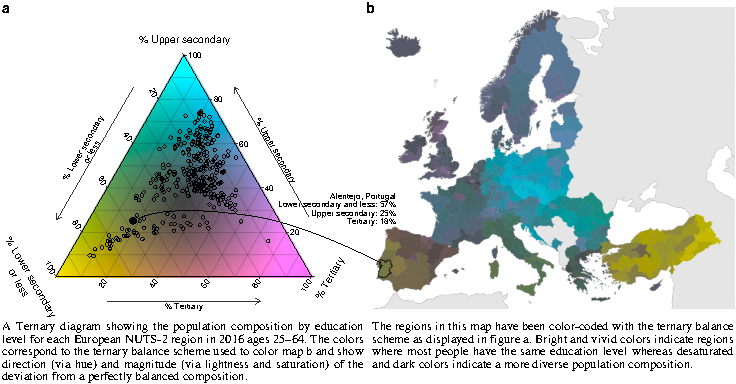
\includegraphics{figure1.pdf}
\caption{\label{fig:unnamed-chunk-2}Demonstration of the ternary balance scheme showing the composition of educational attainment by region in Europe 2016. Data by Eurostat.}
\end{figure}

\begin{figure}
\centering
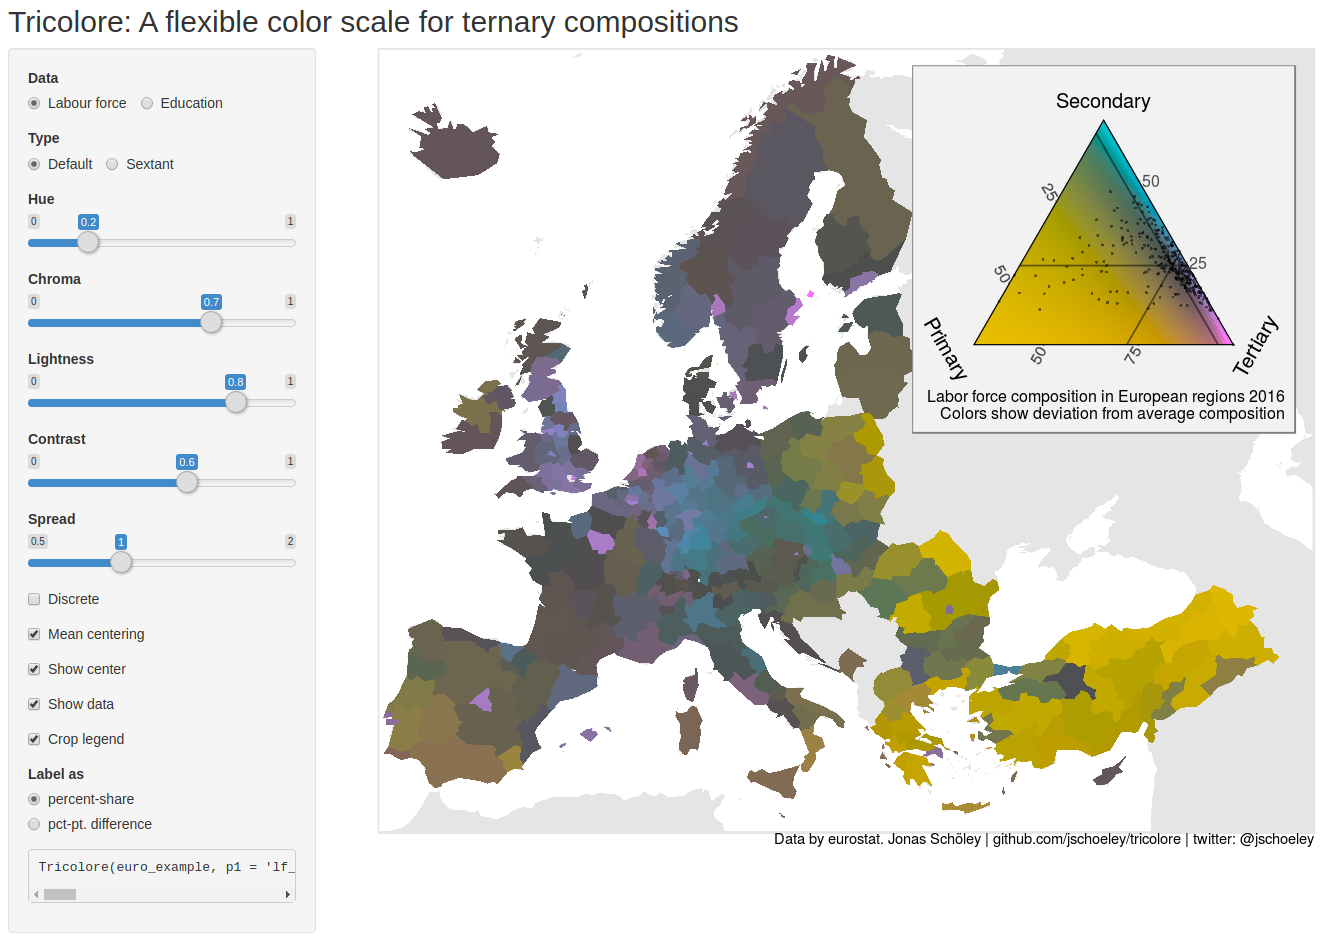
\includegraphics{figure2.png}
\caption{The ``tricolore'' package for the statistical programming language R implements the centered ternary balance color scheme and provides a user interface for quickly testing different parametrizations.}
\end{figure}

\begin{table}

\caption{\label{tab:unnamed-chunk-3}A table with a caption that stretches across two lines. Nearly there... Done. Does it align nicely?}
\centering
\begin{tabular}[t]{rrrrl}
\toprule
Sepal.Length & Sepal.Width & Petal.Length & Petal.Width & Species\\
\midrule
5.1 & 3.5 & 1.4 & 0.2 & setosa\\
4.9 & 3.0 & 1.4 & 0.2 & setosa\\
4.7 & 3.2 & 1.3 & 0.2 & setosa\\
4.6 & 3.1 & 1.5 & 0.2 & setosa\\
5.0 & 3.6 & 1.4 & 0.2 & setosa\\
\addlinespace
5.4 & 3.9 & 1.7 & 0.4 & setosa\\
\bottomrule
\end{tabular}
\end{table}

\hypertarget{equations}{%
\section{Equations}\label{equations}}

Given the observed death counts \(D_{jk}\) in age group \(j\) and stratum \(k\) and associated person-days of exposure to risk \(O_{jk}\) I fit the model

\begin{equation}
  \begin{aligned}
    D_{jk} &\sim \text{Pois}\left(\lambda_{jk}O_{jk}\right) \\
    \lambda_{jk} &= e^{\beta_{0k} +
    \beta_{1k}\log(x_{jk}+1) +
    \beta_{2k}\log^2(x_{jk}+1)},
  \end{aligned}
\label{eq:themodel}
\end{equation}

where \(\lambda_{jk}\) are mortality rates by age group and stratum. For each stratum, a smooth hazard is recovered by evaluating \(\lambda_{jk}\) over a continuous range of ages \(x\).

The stratum specific coefficients \(\beta_{0k}\), \(\beta_{1k}\), \(\beta_{2k}\) are sums of baseline coefficients \(\beta\), prematurity effects \(\beta^\text{Pm}\), prematurity-birth weight interactions \(\beta^{\text{Pm}\times\text{Bw}}\), and prematurity-birth weight-Apgar interactions \(\beta^{\text{Pm}\times\text{Bw}\times\text{Ap}}\) resulting in the multilevel structure

\[
\left(\begin{aligned}
\beta_{0k} \\
\beta_{1k} \\
\beta_{2k}
\end{aligned}\right) =
\underbrace{\left(\begin{aligned}
\beta_0 \\
\beta_1 \\
\beta_2
\end{aligned}\right)}_{\substack{\text{lvl 0} \\ \text{ baseline coef.}}} +
\underbrace{\left(\begin{aligned}
\beta_{0,p[k]}^\text{Pm} \\
\beta_{1,p[k]}^\text{Pm} \\
\beta_{2,p[k]}^\text{Pm}
\end{aligned}\right)}_{\substack{\text{lvl 1} \\ \text{ deviations by} \\ \text{prematurity}}} +
\underbrace{\left(\begin{aligned}
\beta_{0,p[k],b[k]}^{\text{Pm}\times\text{Bw}} \\
\beta_{1,p[k],b[k]}^{\text{Pm}\times\text{Bw}} \\
\beta_{2,p[k],b[k]}^{\text{Pm}\times\text{Bw}}
\end{aligned}\right)}_{\substack{\text{lvl 2} \\ \text{ deviations by} \\ \text{birth weight given} \\ \text{prematurity}}} +
\underbrace{\left(\begin{aligned}
\beta_{0,p[k],b[k],a[k]}^{\text{Pm}\times\text{Bw}\times\text{Ap}} \\
\beta_{1,p[k],b[k],a[k]}^{\text{Pm}\times\text{Bw}\times\text{Ap}} \\
\beta_{2,p[k],b[k],a[k]}^{\text{Pm}\times\text{Bw}\times\text{Ap}}
\end{aligned}\right)}_{\substack{\text{lvl 3} \\ \text{ deviations by} \\ \text{Apgar given} \\ \text{prematurity and} \\ \text{birth weight}}},
\]

where \(p[k], b[k]\) and \(a[k]\) denote the prematurity, birth weight and Apgar level associated with stratum \(k\). Except for the baseline \(\beta\)'s each set of coefficients is assumed to be drawn from a multivariate-Normal distribution with zero mean and covariance matrix

\[
\Sigma = \begin{pmatrix}
    \sigma^2_{\beta_0} & \sigma_{\beta_0\beta_1} & \sigma_{\beta_0\beta_2} \\
    \sigma_{\beta_0\beta_1} & \sigma^2_{\beta_1} & \sigma_{\beta_1\beta_2} \\
    \sigma_{\beta_0\beta_2} & \sigma_{\beta_1\beta_2} & \sigma^2_{\beta_2}
    \end{pmatrix},
\]

with separate estimates for levels one to three.

\hypertarget{lists}{%
\section{Lists}\label{lists}}

\begin{itemize}
\tightlist
\item
  Ringo

  \begin{itemize}
  \tightlist
  \item
    Drums
  \end{itemize}
\item
  George

  \begin{itemize}
  \tightlist
  \item
    Guitar
  \end{itemize}
\item
  Paul

  \begin{itemize}
  \tightlist
  \item
    Bass
  \item
    Piano
  \end{itemize}
\item
  John

  \begin{itemize}
  \tightlist
  \item
    Guitar
  \item
    Piano
  \end{itemize}
\end{itemize}

\hypertarget{section}{%
\section{Section}\label{section}}

\hypertarget{subsection}{%
\subsection{Subsection}\label{subsection}}

\hypertarget{subsubsection}{%
\subsubsection{Subsubsection}\label{subsubsection}}

\hypertarget{acknowledgments}{%
\section{Acknowledgments}\label{acknowledgments}}

I'd like to thank my husband whose caring love allowed me to fully concentrate on my work.

%--- Print references --------------------------------------------------

\newpage

\addcontentsline{toc}{section}{\numberline{}References}

\bibliography{references.bib}

%--- Print appendix ----------------------------------------------------

% total number of appendices
\newcounter{totalappendixcount}  \stepcounter{totalappendixcount}  \stepcounter{totalappendixcount} 
% loop iterator
\newcounter{currentappendixcount}

% add appendices

 \stepcounter{currentappendixcount}
 % if only a single appendix use a different labeling scheme
 \ifnum\value{totalappendixcount}=1
   \def \currentappendixlabel {}
   \def \currentappendixfloatlabel {A}
 \else
   \def \currentappendixlabel {\Alph{currentappendixcount}}
   \def \currentappendixfloatlabel {\Alph{currentappendixcount}}
 \fi

  \clearpage
  \section*{Appendix \currentappendixlabel}\FloatBarrier
  \addcontentsline{toc}{section}{\numberline{}Appendix \currentappendixlabel}
  \setcounter{section}{0}
  \renewcommand{\thesection}{\currentappendixfloatlabel-\arabic{section}}
  \setcounter{figure}{0}
  \renewcommand{\thefigure}{\currentappendixfloatlabel-\arabic{figure}}
  \setcounter{table}{0}
  \renewcommand{\thetable}{\currentappendixfloatlabel-\arabic{table}}

  \begin{Shaded}
\begin{Highlighting}[]
\CommentTok{\#\textquotesingle{} Get Stratified Life{-}table From Survival Data}
\CommentTok{\#\textquotesingle{}}
\CommentTok{\#\textquotesingle{} Aggregate individual level survival data into a stratified}
\CommentTok{\#\textquotesingle{} life{-}tables with prespecified age{-}groups using the assumptions of}
\CommentTok{\#\textquotesingle{} piecewise{-}constant hazards.}
\CommentTok{\#\textquotesingle{}}
\CommentTok{\#\textquotesingle{} @param df a data frame}
\CommentTok{\#\textquotesingle{} @param x time at censoring or event}
\CommentTok{\#\textquotesingle{} @param event event indicator, 0 if censoring, 1 if event}
\CommentTok{\#\textquotesingle{} @param cuts vector of cuts for life{-}table age groups}
\CommentTok{\#\textquotesingle{} @param ... strata}
\CommentTok{\#\textquotesingle{}}
\CommentTok{\#\textquotesingle{} @author Jonas Schöley}
\NormalTok{GetLifeTable }\OtherTok{\textless{}{-}} \ControlFlowTok{function}\NormalTok{ (df, x, event, cuts, ...) \{}

\NormalTok{  x\_i }\OtherTok{=} \FunctionTok{enquo}\NormalTok{(x); event\_i }\OtherTok{=} \FunctionTok{enquo}\NormalTok{(event); strata }\OtherTok{=} \FunctionTok{enexprs}\NormalTok{(...)}

\NormalTok{  lt }\OtherTok{\textless{}{-}}
\NormalTok{    df }\SpecialCharTok{\%\textgreater{}\%}
    \CommentTok{\# aggregate individual level event and censoring times}
    \CommentTok{\# into predefined age groups}
    \FunctionTok{mutate}\NormalTok{(}
      \AttributeTok{j =}
        \FunctionTok{.bincode}\NormalTok{(}
          \AttributeTok{x =} \SpecialCharTok{!!}\NormalTok{x\_i, }\AttributeTok{breaks =}\NormalTok{ cuts,}
          \CommentTok{\# [a, b)}
          \AttributeTok{right =} \ConstantTok{FALSE}\NormalTok{, }\AttributeTok{include.lowest =} \ConstantTok{FALSE}
\NormalTok{        ),}
      \AttributeTok{x\_jk =}
\NormalTok{        cuts[j]}
\NormalTok{    ) }\SpecialCharTok{\%\textgreater{}\%}
    \FunctionTok{group\_by}\NormalTok{(}\SpecialCharTok{!!!}\NormalTok{strata, j, x\_jk) }\SpecialCharTok{\%\textgreater{}\%}
    \FunctionTok{summarise}\NormalTok{(}
      \CommentTok{\# total observed deaths in interval}
      \AttributeTok{D\_jk =} \FunctionTok{sum}\NormalTok{(}\SpecialCharTok{!!}\NormalTok{event\_i),}
      \CommentTok{\# total observed censorings in interval}
      \AttributeTok{C\_jk =} \FunctionTok{sum}\NormalTok{(}\SpecialCharTok{!}\NormalTok{(}\SpecialCharTok{!!}\NormalTok{event\_i)),}
      \CommentTok{\# average time spent in interval for}
      \CommentTok{\# those who leave during interval (by death or censoring)}
      \AttributeTok{a\_jk =} \FunctionTok{mean}\NormalTok{(}\SpecialCharTok{!!}\NormalTok{x\_i }\SpecialCharTok{{-}} \FunctionTok{first}\NormalTok{(x\_jk))}
\NormalTok{    ) }\SpecialCharTok{\%\textgreater{}\%}
    \FunctionTok{ungroup}\NormalTok{() }\SpecialCharTok{\%\textgreater{}\%}
    \CommentTok{\# add predefined age intervals to table where no deaths or}
    \CommentTok{\# censorings occoured}
    \FunctionTok{complete}\NormalTok{(}
      \FunctionTok{nesting}\NormalTok{(}\AttributeTok{x\_jk =} \FunctionTok{head}\NormalTok{(cuts, }\SpecialCharTok{{-}}\DecValTok{1}\NormalTok{), }\AttributeTok{j =} \DecValTok{1}\SpecialCharTok{:}\FunctionTok{length}\NormalTok{(}\FunctionTok{head}\NormalTok{(cuts, }\SpecialCharTok{{-}}\DecValTok{1}\NormalTok{))),}
      \FunctionTok{nesting}\NormalTok{(}\SpecialCharTok{!!!}\NormalTok{strata),}
      \AttributeTok{fill =} \FunctionTok{list}\NormalTok{(}\AttributeTok{D\_jk =} \DecValTok{0}\NormalTok{, }\AttributeTok{C\_jk =} \DecValTok{0}\NormalTok{, }\AttributeTok{a\_jk =} \ConstantTok{NA}\NormalTok{)}
\NormalTok{    ) }\SpecialCharTok{\%\textgreater{}\%}
    \FunctionTok{arrange}\NormalTok{(}\SpecialCharTok{!!!}\NormalTok{strata, x\_jk) }\SpecialCharTok{\%\textgreater{}\%}
    \FunctionTok{mutate}\NormalTok{(}
      \AttributeTok{k =} \FunctionTok{group\_indices}\NormalTok{(., }\SpecialCharTok{!!!}\NormalTok{strata)}
\NormalTok{    ) }\SpecialCharTok{\%\textgreater{}\%}
    \FunctionTok{group\_by}\NormalTok{(k) }\SpecialCharTok{\%\textgreater{}\%}
    \CommentTok{\# calculate life{-}table}
    \FunctionTok{mutate}\NormalTok{(}
      \CommentTok{\# width of the interval}
      \AttributeTok{n\_jk =}
        \FunctionTok{c}\NormalTok{(}\FunctionTok{diff}\NormalTok{(x\_jk), }\FunctionTok{last}\NormalTok{(cuts)}\SpecialCharTok{{-}}\FunctionTok{last}\NormalTok{(x\_jk)),}
      \CommentTok{\# observed population alive at start of interval}
      \AttributeTok{N\_jk =}
        \FunctionTok{head}\NormalTok{(}\FunctionTok{cumsum}\NormalTok{(}\FunctionTok{c}\NormalTok{(}\FunctionTok{sum}\NormalTok{(C\_jk}\SpecialCharTok{+}\NormalTok{D\_jk), }\SpecialCharTok{{-}}\NormalTok{(C\_jk}\SpecialCharTok{+}\NormalTok{D\_jk))), }\SpecialCharTok{{-}}\DecValTok{1}\NormalTok{),}
      \CommentTok{\# total person{-}time of exposure over interval}
      \AttributeTok{O\_jk =}
\NormalTok{        (N\_jk}\SpecialCharTok{{-}}\NormalTok{D\_jk}\SpecialCharTok{{-}}\NormalTok{C\_jk)}\SpecialCharTok{*}\NormalTok{n\_jk }\SpecialCharTok{+}
        \FunctionTok{ifelse}\NormalTok{(}\FunctionTok{is.na}\NormalTok{(a\_jk), }\DecValTok{0}\NormalTok{, a\_jk}\SpecialCharTok{*}\NormalTok{(D\_jk}\SpecialCharTok{+}\NormalTok{C\_jk)),}
      \CommentTok{\# mortality rate over interval}
      \AttributeTok{m\_jk =}
        \FunctionTok{ifelse}\NormalTok{(O\_jk }\SpecialCharTok{==} \DecValTok{0}\NormalTok{, }\DecValTok{0}\NormalTok{, D\_jk}\SpecialCharTok{/}\NormalTok{O\_jk),}
      \CommentTok{\# probability of surviving interval}
      \CommentTok{\# assuming constant force of mortality}
      \AttributeTok{p\_jk =}
        \FunctionTok{exp}\NormalTok{(}\SpecialCharTok{{-}}\NormalTok{m\_jk}\SpecialCharTok{*}\NormalTok{n\_jk),}
      \CommentTok{\# probability of death during the interval given survival}
      \CommentTok{\# to interval}
      \AttributeTok{q\_jk =}
        \DecValTok{1}\SpecialCharTok{{-}}\NormalTok{p\_jk,}
      \CommentTok{\# probability of survival until interval start}
      \AttributeTok{l\_jk =}
        \FunctionTok{cumprod}\NormalTok{(}\FunctionTok{c}\NormalTok{(}\DecValTok{1}\NormalTok{, }\FunctionTok{head}\NormalTok{(p\_jk, }\SpecialCharTok{{-}}\DecValTok{1}\NormalTok{))),}
      \CommentTok{\# probability of death in interval}
      \AttributeTok{d\_jk =}
        \FunctionTok{c}\NormalTok{(}\SpecialCharTok{{-}}\FunctionTok{diff}\NormalTok{(l\_jk), }\FunctionTok{last}\NormalTok{(l\_jk)}\SpecialCharTok{*}\FunctionTok{last}\NormalTok{(q\_jk))}
\NormalTok{    ) }\SpecialCharTok{\%\textgreater{}\%}
    \CommentTok{\# distribution of stratum{-}specific exposures by age}
    \FunctionTok{group\_by}\NormalTok{(j) }\SpecialCharTok{\%\textgreater{}\%}
    \FunctionTok{mutate}\NormalTok{(}
      \AttributeTok{pi\_jk =}\NormalTok{ O\_jk}\SpecialCharTok{/}\FunctionTok{sum}\NormalTok{(O\_jk)}
\NormalTok{    ) }\SpecialCharTok{\%\textgreater{}\%}
    \FunctionTok{ungroup}\NormalTok{() }\SpecialCharTok{\%\textgreater{}\%}
    \FunctionTok{select}\NormalTok{(}
\NormalTok{      k, j, }\SpecialCharTok{!!!}\NormalTok{strata, x\_jk, n\_jk, N\_jk, a\_jk, O\_jk, D\_jk, C\_jk,}
\NormalTok{      m\_jk, q\_jk, l\_jk, d\_jk, pi\_jk}
\NormalTok{    )}

  \FunctionTok{return}\NormalTok{(lt)}

\NormalTok{\}}
\end{Highlighting}
\end{Shaded}



 \stepcounter{currentappendixcount}
 % if only a single appendix use a different labeling scheme
 \ifnum\value{totalappendixcount}=1
   \def \currentappendixlabel {}
   \def \currentappendixfloatlabel {A}
 \else
   \def \currentappendixlabel {\Alph{currentappendixcount}}
   \def \currentappendixfloatlabel {\Alph{currentappendixcount}}
 \fi

  \clearpage
  \section*{Appendix \currentappendixlabel}\FloatBarrier
  \addcontentsline{toc}{section}{\numberline{}Appendix \currentappendixlabel}
  \setcounter{section}{0}
  \renewcommand{\thesection}{\currentappendixfloatlabel-\arabic{section}}
  \setcounter{figure}{0}
  \renewcommand{\thefigure}{\currentappendixfloatlabel-\arabic{figure}}
  \setcounter{table}{0}
  \renewcommand{\thetable}{\currentappendixfloatlabel-\arabic{table}}

  \begin{Shaded}
\begin{Highlighting}[]
\FunctionTok{plot}\NormalTok{(cars)}
\end{Highlighting}
\end{Shaded}

  \begin{figure}
  \centering
  \includegraphics{example_files/figure-latex/unnamed-chunk-1-1.pdf}
  \caption{\label{fig:unnamed-chunk-1}The cars data set}
  \end{figure}


%--- End document ------------------------------------------------------

\cleardoublepage

\end{document}
